\documentclass{article}
\usepackage{graphicx}
\usepackage{geometry}
\geometry{margin=1in}

\begin{document}

% ---------------- LOGO ----------------
\begin{center}

\includegraphics[width=3cm]{iiitb_comet_logo.jpg}

\vspace{0.3cm}

\textbf{Name: Srinidhi A} \\
\textbf{ID: COMETFWC053}
\end{center}

\vspace{0.5cm}

% ---------------- HEADING ----------------
\begin{center}
\Large \textbf{GATE Question no. 59}
\end{center}

\vspace{0.5cm}

% ---------------- QUESTION ----------------
\section*{Question}

Two products are sold from a vending machine, which has two push buttons $P_1$ and $P_2$. When a button is pressed, the price of the corresponding product is displayed in a 7-segment display.

\begin{itemize}
\item If no buttons are pressed, `0' is displayed, signifying Rs. 0.
\item If only $P_1$ is pressed, `2' is displayed, signifying Rs. 2.
\item If only $P_2$ is pressed, `5' is displayed, signifying Rs. 5.
\item If both $P_1$ and $P_2$ are pressed, `E' is displayed, signifying Error.
\end{itemize}

Consider:
\begin{itemize}
\item push button pressed/not pressed is equivalent to logic 1/0 respectively.
\item a segment glowing/not glowing in the display is equivalent to logic 1/0 respectively.
\end{itemize}

If the segment $g$ and $d$ are considered as functions of $P_1$ and $P_2$, determine the correct logic expressions.


\begin{figure}[h]
\centering
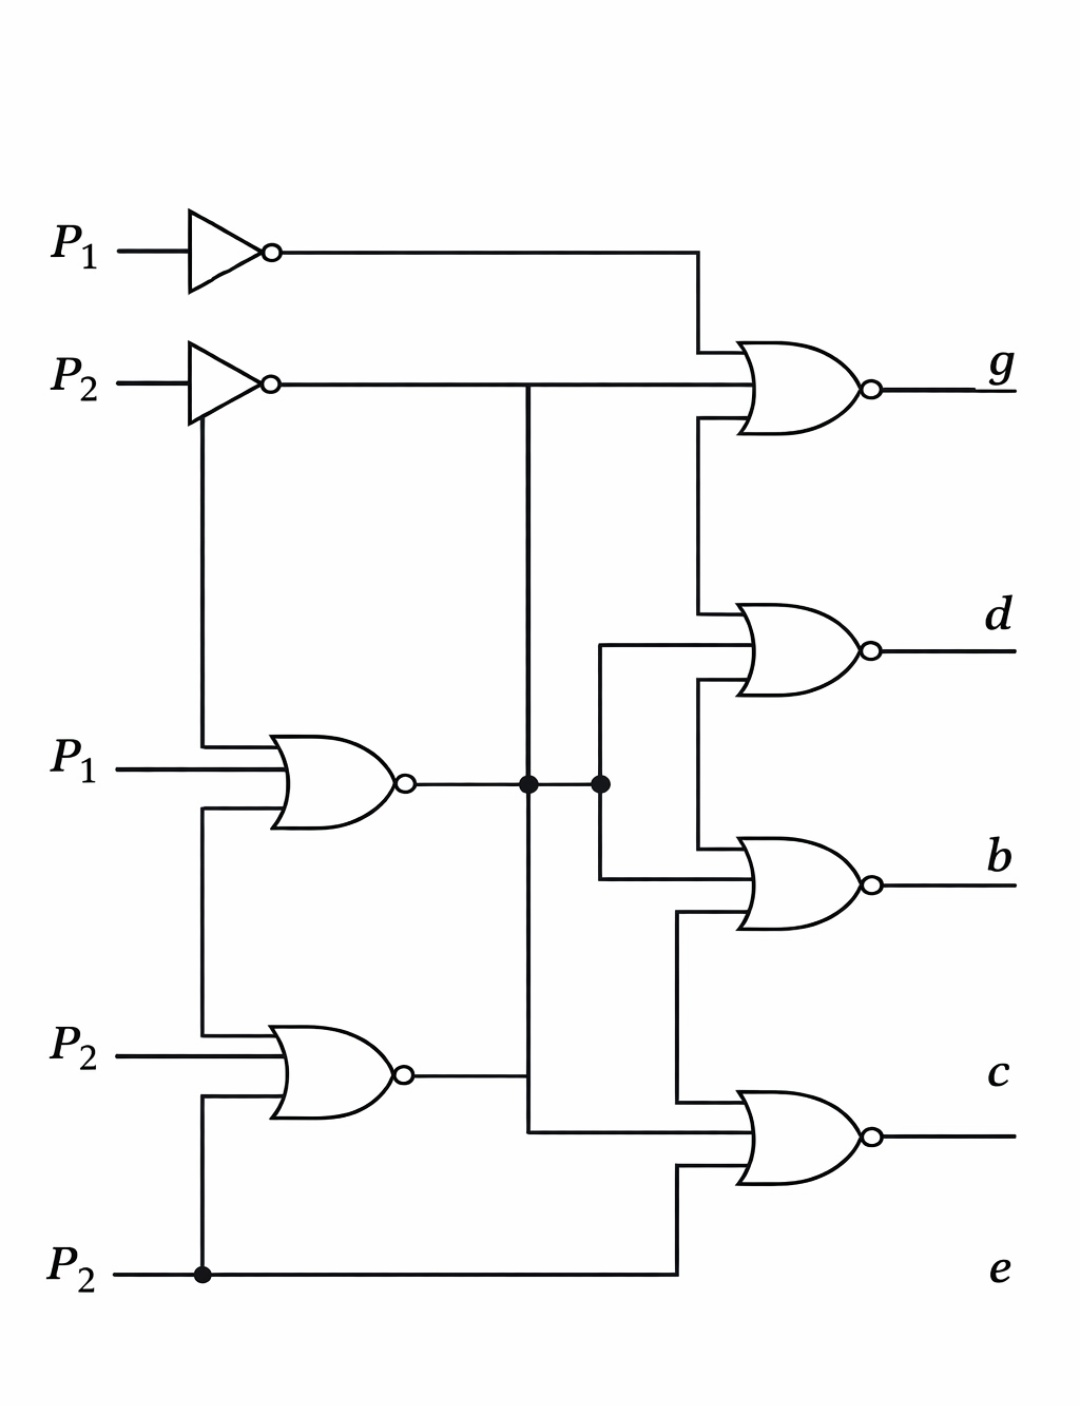
\includegraphics[width=0.5\textwidth]{question.jpg}
\caption{GATE EC 2009 Question 59}
\end{figure}

% ---------------- QUESTION ANALYSIS ----------------
\section*{Question Analysis}

Inputs: $P_1$, $P_2$

Push button pressed = Logic 1  
Push button not pressed = Logic 0  

Display outputs:

\begin{itemize}
\item No button pressed → 0
\item Only $P_1$ pressed → 2
\item Only $P_2$ pressed → 5
\item Both pressed → E
\end{itemize}

We derive expressions for required segments.

Example:

Segment $g = P_1 + P_2$

Segment $d = c + e$

% ---------------- TRUTH TABLE ----------------
\section*{Truth Table}

\begin{center}
\begin{tabular}{|c|c|c|}
\hline
$P_1$ & $P_2$ & Display \\
\hline
0 & 0 & 0 \\
0 & 1 & 5 \\
1 & 0 & 2 \\
1 & 1 & E \\
\hline
\end{tabular}
\end{center}

% ---------------- HARDWARE IMPLEMENTATION ----------------
\section*{Hardware Implementation}

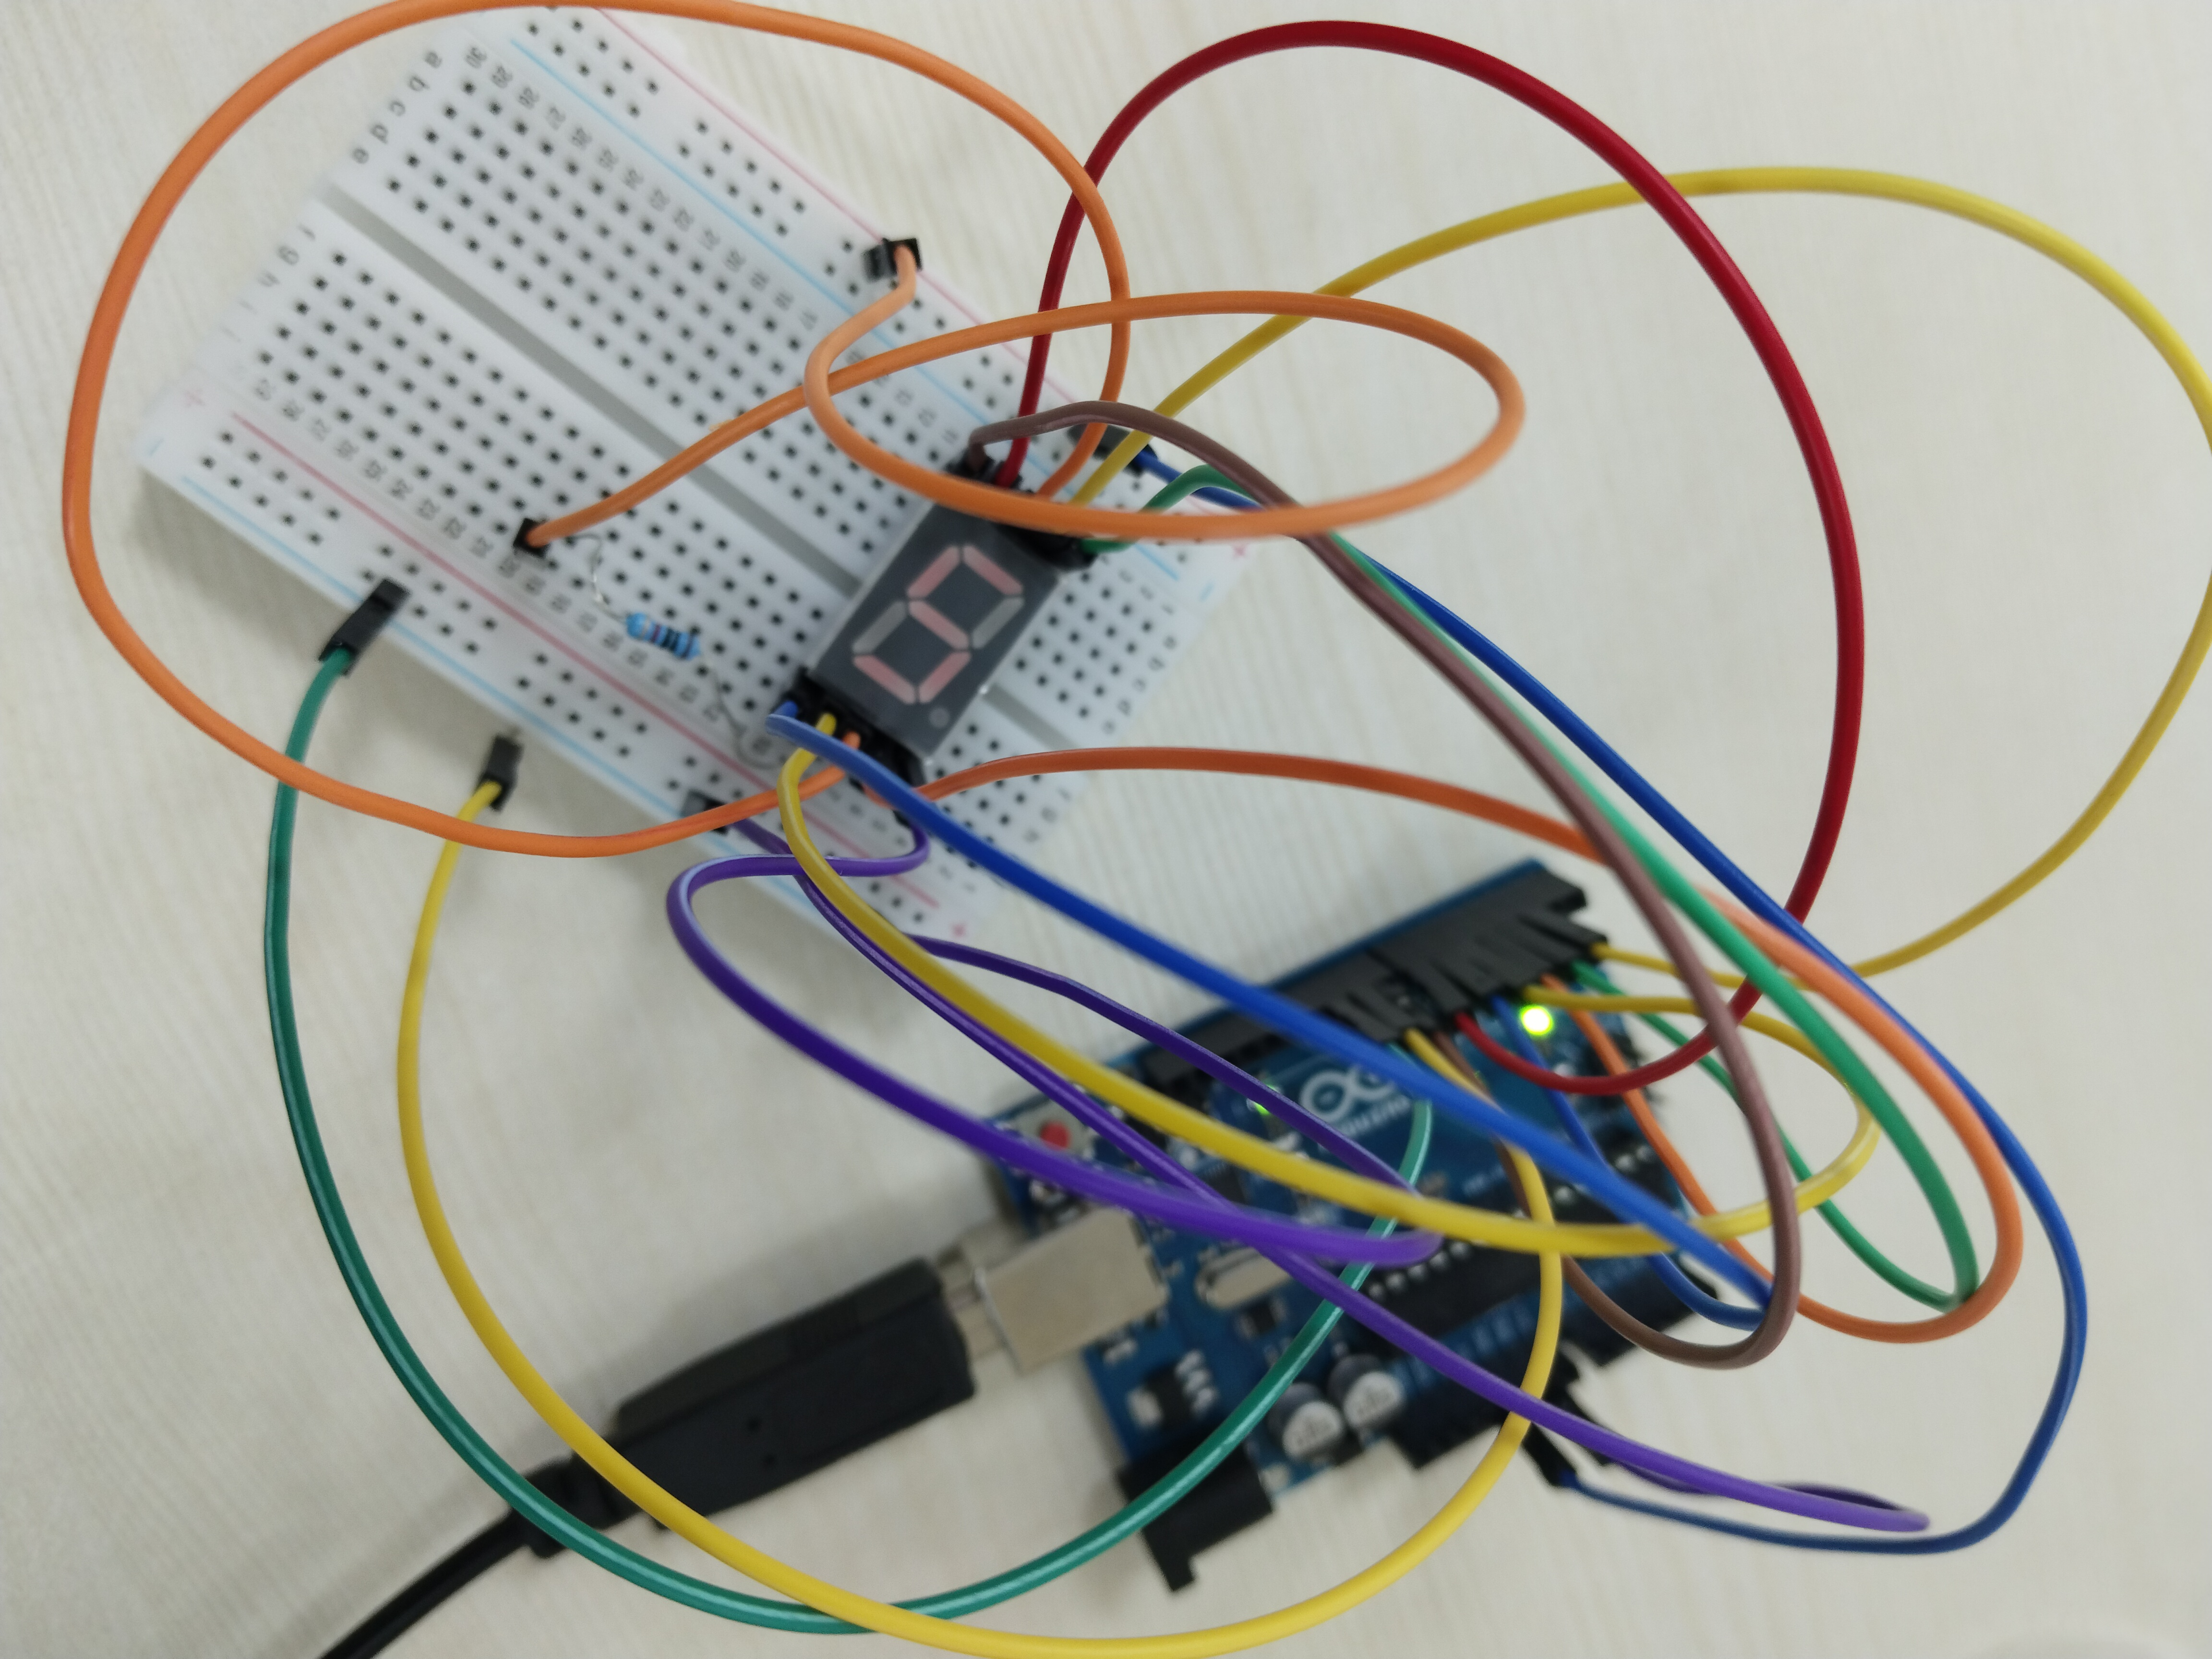
\includegraphics[width=\textwidth]{hardware.jpg}

% ---------------- REQUIRED COMPONENTS ----------------
\section*{Required Components}

\begin{itemize}
\item Arduino UNO
\item Breadboard
\item 7-segment display
\item Push buttons (2)
\item Resistors
\item Connecting wires
\item OTG cable
\end{itemize}

% ---------------- PIN CONNECTIONS ----------------
\section*{Pin Connections}

\begin{itemize}
\item Segment a → Pin 2
\item Segment b → Pin 3
\item Segment c → Pin 4
\item Segment d → Pin 5
\item Segment e → Pin 6
\item Segment f → Pin 7
\item Segment g → Pin 8
\item $P_1$ → Pin 9
\item $P_2$ → Pin 10
\end{itemize}

% ---------------- LOGIC DESCRIPTION ----------------
\section*{Logic Description}

The push buttons control the display output.  
Depending on $P_1$ and $P_2$, the corresponding segments glow to display 0, 2, 5 or E.

Logic expressions are implemented using OR and NOT gates.

% ---------------- CODE UPLOADING STEPS ----------------
\section*{Code Uploading Steps}

\begin{enumerate}
\item Create a Platform IO project.
\item Write the code in \texttt{main.cpp} inside \texttt{src}.
\item Run the PIO project using command: \texttt{pio run}.
\item It compiles the code and creates a \texttt{.hex} file.
\item Copy the hex file to ArduinoDroid folder.
\item Connect Arduino UNO to mobile using OTG cable.
\item Upload using "Upload precompiled" option.
\item Observe the output and verify the expression.
\end{enumerate}

% ---------------- EXPERIMENTAL TRUTH TABLE ----------------
\section*{Experimental Truth Table}

\begin{center}
\begin{tabular}{|c|c|c|}
\hline
$P_1$ & $P_2$ & Observed Output \\
\hline
0 & 0 & 0 \\
0 & 1 & 5 \\
1 & 0 & 2 \\
1 & 1 & E \\
\hline
\end{tabular}
\end{center}

% ---------------- CONCLUSION ----------------
\section*{Conclusion}

The logic for GATE Question 59 was successfully implemented using Arduino UNO and 7-segment display.  
The experimental results match the theoretical truth table.

\end{document}
